\definecolor{Espresso}{HTML}{3B2F2F}
\definecolor{Cream}{HTML}{FFF7EA}
\definecolor{Sand}{HTML}{F1D6B8}
\definecolor{Terracotta}{HTML}{C96F4A}
\definecolor{Olive}{HTML}{7D8B52}
\definecolor{Plum}{HTML}{6F4E7C}
\definecolor{organiserblue}{HTML}{2E6F9E}

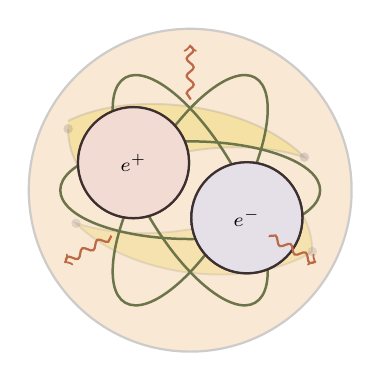
\begin{tikzpicture}[
  x=1cm,y=1cm,
  particle/.style={circle,draw=Espresso,line width=0.8pt,minimum size=1.41cm,inner sep=0pt,font=\scriptsize\bfseries},
  orbit/.style={draw=Olive!75!Espresso,line width=0.9pt},
  photon/.style={decorate,decoration={snake,amplitude=0.45mm,segment length=2.2mm},line width=0.8pt,Terracotta!90!Espresso}
]
  \fill[Sand!45!Cream] (0,0) circle (2.05);
  \draw[Espresso!25,line width=0.8pt] (0,0) circle (2.05);

  \begin{scope}[opacity=0.25]
    \fill[Terracotta!35!yellow]
      (-1.55,0.88)
      .. controls (-0.75,1.28) and (0.75,1.12) .. (1.45,0.42)
      .. controls (0.62,0.68) and (-0.42,0.52) .. (-1.20,0.08)
      .. controls (-1.42,0.22) and (-1.55,0.48) .. (-1.55,0.78)
      -- cycle;
    \draw[Espresso!55,line width=0.7pt]
      (-1.55,0.88)
      .. controls (-0.75,1.28) and (0.75,1.12) .. (1.45,0.42)
      .. controls (0.62,0.68) and (-0.42,0.52) .. (-1.20,0.08)
      .. controls (-1.42,0.22) and (-1.55,0.48) .. (-1.55,0.78);
    \fill[Espresso!65] (-1.55,0.78) circle (0.06);
    \fill[Espresso!65] (1.45,0.42) circle (0.06);
  \end{scope}

  \begin{scope}[opacity=0.2,rotate=180]
    \fill[Terracotta!35!yellow]
      (-1.55,0.78)
      .. controls (-0.75,1.28) and (0.75,1.12) .. (1.45,0.42)
      .. controls (0.62,0.68) and (-0.42,0.52) .. (-1.20,0.08)
      .. controls (-1.42,0.22) and (-1.55,0.48) .. (-1.55,0.78)
      -- cycle;
    \draw[Espresso!55,line width=0.7pt]
      (-1.55,0.78)
      .. controls (-0.75,1.28) and (0.75,1.12) .. (1.45,0.42)
      .. controls (0.62,0.68) and (-0.42,0.52) .. (-1.20,0.08)
      .. controls (-1.42,0.22) and (-1.55,0.48) .. (-1.55,0.78);
    \fill[Espresso!65] (-1.55,0.78) circle (0.06);
    \fill[Espresso!65] (1.45,0.42) circle (0.06);
  \end{scope}

  \draw[orbit,rotate=0] (0,0) ellipse (1.65 and 0.62);
  \draw[orbit,rotate=60] (0,0) ellipse (1.65 and 0.62);
  \draw[orbit,rotate=-60] (0,0) ellipse (1.65 and 0.62);

  \shade[ball color=Terracotta!85!white] (-0.72,0.35) circle (0.72);
  \node[particle,fill=Terracotta!25] at (-0.72,0.35) {$e^+$};

  \shade[ball color=Plum!75!white] (0.72,-0.35) circle (0.72);
  \node[particle,fill=Plum!18] at (0.72,-0.35) {$e^-$};

  % \node[font=\scriptsize\bfseries,Espresso] at (0,-2.45) {positronium};
  % \node[font=\scriptsize,Espresso,align=center] at (0,-2.85) {bound state of\\electron and positron};

  % Three emitted photons at 120 degrees: net momentum is zero.
  \draw[photon,<-] (0,1.85) -- (0,1.15);
  \draw[photon,<-] (-1.60,-0.92) -- (-1.00,-0.58);
  \draw[photon,<-] (1.60,-0.92) -- (1.00,-0.58);
\end{tikzpicture}